% ------------------------------------------------------------------
\renewcommand{\thisweek}{MATH327 Week 11}
\renewcommand{\moddate}{Last modified 5 May 2021}
\setcounter{section}{11}
\setcounter{subsection}{0}
\phantomsection
\addcontentsline{toc}{section}{Week 11: Synthesis and broader applications}
\section*{Week 11: Synthesis and broader applications}
\subsection{Monte Carlo importance sampling}
Last week we wrapped up our discussion of the mean-field approximation to the Ising model by comparing some of its predictions against results from numerical computations for systems in $d \geq 3$ dimensions where no exact solution is known.
These numerical results may have come as a surprise given the statement at the end of \secref{sec:Ising} that numerically evaluating the Ising model partition function even for tiny systems with $N \sim 1000$ spins is far beyond the capabilities of existing or foreseeable supercomputers.
To quantify `tiny', consider that $N \sim 1000$ would correspond to a $10\times 10\times 10$ lattice in three dimensions or a $6\times 6\times 6\times 6$ lattice in four dimensions, both very far from the thermodynamic limit of interest for phase transitions.

The key is that practical numerical computations do not perform a `brute-force' evaluation of every single micro-state that is summed over in the formal definition of the partition function (and hence in the expectation values that we have derived from the partition function).
Instead, they proceed by (pseudo-)randomly selecting (or \textbf{sampling}) a small subset of those micro-states, and using this subset to compute results for the average energy, magnetization, and other thermodynamic quantities.
The law of large numbers allows us to treat these averages as controlled approximations to the true ensemble expectation values.

As we saw in the computer project, such numerical calculations employ pseudo-random numbers rather than complete randomness, which allows them to be reproducible up to very high precision by different people using different computers.
Due to the role of randomness, these numerical approaches have become known as \textbf{Monte Carlo} methods, based on a whimsical reference to the famous gambling centre in Monaco.
Monte Carlo methods are crucial in statistical physics because they are applicable even to the interacting systems introduced last week, where there are no longer dramatic simplifications from factorization.

An intuitive illustration of how Monte Carlo methods work is provided by using them to numerically evaluate integrals.
The idea is that the integral can be numerically approximated by evaluating its integrand at randomly sampled points in the integration domain, and normalizing by the number of samples.
A simple example is to compute
\begin{align*}
  \int_{-1}^1 dx \int_{-1}^1 dy \ H\!\left(1 - \left\{x^2 + y^2\right\}\right) & = \pi \qquad &
  H(r) & = \left\{\begin{array}{l}1 \qquad \mbox{for } \ r \geq 0 \\
                                  0 \qquad \mbox{for } \ r < 0\end{array}\right. ,
\end{align*}
which is just the area of a disk with radius $R = 1$, in a square integration domain with area $4$, as shown below.
Since the integrand is either $0$ or $1$ for each randomly sampled point in that domain, simply counting the fraction of the $S$ samples that lie in the disk provides a numerical determination of $\pi$, with a \textit{statistical uncertainty} that vanishes $\sim 1 / \sqrt{S}$.
In just a few minutes, \href{https://github.com/daschaich/MATH327_2021/blob/master/lecture_notes/week11_pi.py}{this Python code} predicts $\pi = 3.14155 \pm 0.00024$ purely from the statistics of pseudo-random numbers.

\begin{center}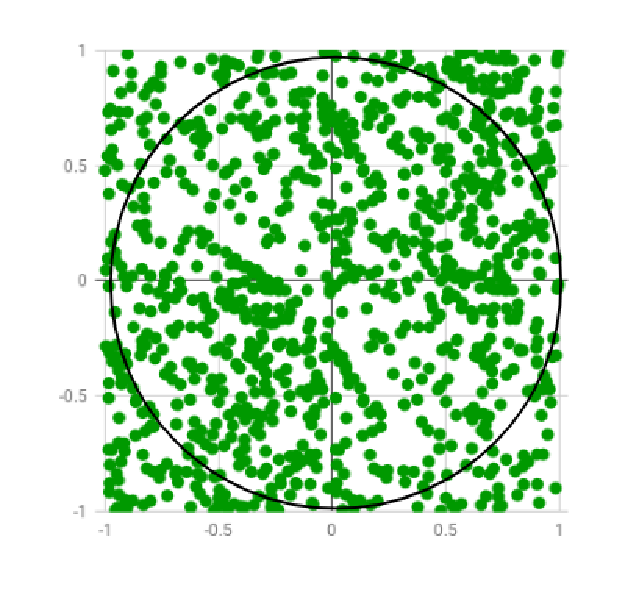
\includegraphics[width=0.6\textwidth]{figs/week11_pi.pdf}\end{center}

Of course, Monte Carlo integration is an extremely inefficient way to determine $\pi$.
These numerical methods are most useful when analytic solutions are not available, and especially for very high-dimensional integrals such as partition functions of statistical systems.
State-of-the-art research in theoretical physics routinely uses Monte Carlo methods to numerically evaluate billion-dimensional integrals.

Switching back to the language of statistical ensembles, there are an enormous number of possible micro-states for any interacting systems of interest, only a vanishingly small fraction of which can be sampled in a reasonable amount of time.
Even if we put in the time to sample a trillion ($10^{12}$) micro-states of the tiny $N \sim 1000$ Ising systems considered above, this would account for only about one part in $10^{288}$ of the total $2^N \sim 10^{300}$ micro-states.
Even worse, as $N$ increases the number of possible Ising model micro-states grows exponentially quickly, $2^N$, and each micro-state takes more work to sample.
For a concrete example, \href{https://arxiv.org/abs/1502.07613}{this research publication} from 2015 includes a calculation with $N \sim 10^9$ that was only able to sample $\sim 10^4$ out of roughly $2^{10^9} \sim 10^{300{,}000{,}000}$ micro-states. % N=64^5~1e9 and log_10(2^(64^5))~3e8

For sufficiently high temperatures, our consideration of the disordered phase of the Ising model in \secref{sec:Ising_phases} suggests that randomly sampling even such a tiny fraction of the micro-states would still suffice.
All of those micro-states are equally probably in the infinite-temperature limit, where we would just need to consider enough samples $S$ to produce reasonably small statistical uncertainties $\sim 1 / \sqrt{S}$.
However, the low-temperature ordered phase is more challenging.
We saw that the large-scale behaviour of the system in this phase is dominated by a very small number of micro-states.
For sufficiently low temperatures, just the two degenerate ground states effectively determine the magnetization, with only exponentially suppressed corrections from higher-energy excited states.
As there is essentially no chance of randomly sampling either of those two ground states, the approach described above seems doomed to fail.

The cure is to carefully guide the procedure so that the probability of sampling a particular micro-state $\om_i$ is proportional to its probability $p_i \propto e^{-\be E_i}$, without introducing any bias.
This is known as \textbf{importance sampling}, since it preferentially samples the important micro-states that make the most significant contributions to the partition function and derived quantities.
As $\be \to \infty$ in the low-temperature phase, the probability of sampling the ground states would be exponentially enhanced, as desired.
As $\be \to 0$ in the high-temperature phase, there would be little change compared to the more straightforward approach described above, since all micro-states would become equally probable.

A challenge facing importance sampling is that the energies $E_i$ are not known in advance.
They are generally only computed for those few micro-states that are sampled.
An ingenious way to get around this challenge\footnote{This approach was developed in 1953 by \href{https://en.wikipedia.org/wiki/Nicholas_Metropolis}{Nick Metropolis}, \href{https://en.wikipedia.org/wiki/Arianna_W._Rosenbluth}{Arianna Rosenbluth}, \href{https://en.wikipedia.org/wiki/Marshall_Rosenbluth}{Marshall Rosenbluth}, \href{https://en.wikipedia.org/wiki/Augusta_H._Teller}{Mici Teller} and \href{https://en.wikipedia.org/wiki/Edward_Teller}{Edward Teller}.  In an infamous misfiring of alphabetical ordering, it remains widely known as the ``Metropolis algorithm'' even though Metropolis's role was providing specialized computing equipment rather than creating the algorithm itself.  In addition, the key contributions of Arianna Rosenbluth and Mici Teller were under-appreciated for many years.} is by incorporating the concept of Markov chains that we encountered all the way back in \secref{sec:diffusion}.
Recall that a Markov chain is a process in which the next micro-state to be sampled is chosen based on the micro-state currently under consideration, with no `memory' of any other micro-states that may already have been sampled.

Applying this to the Ising model, we can begin with any random spin configuration.
Randomly selecting one spin, $s_i$, we compute $\De E_i$, the change in the system's energy that would be caused by flipping $s_i \to -s_i$.
We then update the spin configuration by `accepting' this spin flip with probability
\begin{equation}
  \label{eq:MRTprob}
  P_{\text{accept}} = \mbox{min}\left\{1, e^{-\be \De E}\right\},
\end{equation}
which defines the next micro-state in the Markov chain.
Importantly, this new micro-state may be identical to the previous micro-state with probability $P_{\text{reject}} = 1 - P_{\text{accept}}$.
This is exactly what we would want in the zero-temperature limit where the ground state should dominate.
We then repeat this single-spin update procedure as many times as our computers can handle.

Digging into \eq{eq:MRTprob}, we can see that a spin flip that lowers the energy will always be accepted, since $\De E < 0 \implies e^{-\be \De E} > 1$.
The algorithm is therefore free to approach the minimum-energy ground state of the system.
If it is in the ground state, then any spin flip will increase the energy, $\De E > 0$, and will only be accepted with an exponentially suppressed probability $e^{-\be \De E} \to 0$ as $T = 1 / \be \to 0$, as desired.
More generally, if we consider two micro-states $\om_A$ and $\om_B$ with $E_A \leq E_B$, then the relative probabilities of moving between these two micro-states are
\begin{equation*}
  \frac{P(A \to B)}{P(B \to A)} = \frac{\mbox{min}\left\{1, e^{-\be(E_B - E_A)}\right\}}{\mbox{min}\left\{1, e^{-\be(E_A - E_B)}\right\}} = \frac{e^{-\be(E_B - E_A)}}{1} = \frac{e^{-\be E_B}}{e^{-\be E_A}},
\end{equation*}
confirming that the micro-states $\om_i$ will indeed be sampled with probabilities proportional to the Boltzmann factors $e^{-\be E_i}$ that quantify their importance.

You can find more information about this \textit{Metropolis--Rosenbluth--Teller} algorithm in Section~8.2 of Schroeder's \textit{Introduction to Thermal Physics} (reference~2 in the list of further reading on page~6), including a single-page annotated code applying it to the two-dimensional Ising model.
While this is the most famous and most widely used Monte Carlo algorithm in existence, it is far from the only one.
There is an enormous amount of ongoing research developing, optimizing and applying more elaborate Monte Carlo methods to investigate topics throughout the mathematical sciences and beyond.
In \secref{sec:broad} we will briefly look at some of these broader applications.
First, there is another important concept to introduce, called universality, which helps to explain why interacting statistical systems are so useful to apply to such a diverse range of scientific investigations.
% ------------------------------------------------------------------



% ------------------------------------------------------------------
\subsection{Universality}
In \secref{sec:mean_field} we defined the critical exponent $b$ as the power governing the behaviour of the order parameter $\vev{m} \propto \left(T_c - T\right)^b$ as the temperature $T$ approaches (from below) the critical temperature $T_c$ of the second-order phase transition.
This quantity 

% TODO: 3d Ising model vs.\ liquid--gas...
% TODO: \href{https://en.wikipedia.org/wiki/Leo_Kadanoff}{Leo Kadanoff} and \href{https://en.wikipedia.org/wiki/Kenneth_G._Wilson}{Ken Wilson}...

\TODO{Being written...}
% ------------------------------------------------------------------



% ------------------------------------------------------------------
\newpage
\subsection{\label{sec:broad}Broader applications}
\subsubsection*{Voter models}

\TODO{Being written...}

\subsubsection*{Epidemiology}
% arXiv:2101.11399
% similar to original 1953 calculation summarized on Schroeder page 347...

Larger-scale versions of these epidemiological model simulations provide important input into government deliberations regarding what restrictions (such as lockdowns) should be imposed to mitigate the spread of diseases, and how long these restrictions ought to be maintained.

\TODO{Being written...}

\subsubsection*{Flocking}
% Vicsek model of flocking with first-order phase transition

\TODO{Being written...}
% ------------------------------------------------------------------



% ------------------------------------------------------------------
\newpage
\subsection{Wrap-up recap}

\TODO{Being written...}
% ------------------------------------------------------------------
